% !TEX ROOT = ./distributed_mrf.tex
\section{Introduction}\label{sec:introduction}

With the end of Moore's law, computing power in modern systems increasingly comes in the form of parallel processing resources.  A major obstacle faced by network engineers is how to harness this increasingly parallel computing power for scaling distributed systems \cite{265065, 10.5555/3307441.3307467, 10.1145/2815400.2815423, 10.1145/3098822.3098826, 10.5555/3154630.3154639}.

In horizontally scaled applications, a load balancer dispatches jobs across a fleet of workers that process the jobs in parallel \cite{10.5555/3235491}.  In the context of \emph{web applications}, HTTP load balancers \cite{194966, 211279, 9552525} distribute requests across a swarm of backend web servers.  % by hashing over the source IP address (``sticky sessions'').
% This way, requests from the same client will hit the same backend server, improving request locality.
% Meanwhile, resource state is maintained in a key-value store or a relational database.
Multicore \emph{OS network stacks} \cite{211263, 10.1145/3359989.3365412, 10.1145/3452296.3472914} run multiple instances of the networking logic on different CPUs and leverage the NIC to dispatch packets to CPU cores. % In order to avoid packet reordering and improve CPU cache performance, the NIC typically computes a hash over the packet header fields to select the CPU (RSS, RPS, etc.).
In massive-scale \emph{key-value stores} \cite{ghigoff2021bmc}, the key-space is hashed into multiple shards (partitions) and each shard is assigned to a separate server for processing.  The system's overall goal is to achieve the greatest possible parallel speedup with a given number of workers, in order to minimize the execution time of a single task or maximize the number of completed tasks in a given time period.

Suppose a web app handles 100 requests per second using a single server. As we add another server, we expect a throughput of 200 requests per second. In reality, however, we usually obtain slightly less, and this is worsened as the system is scaled up further. This is because some fraction of most workloads is inherently sequential and, therefore, bound to execute on a single CPU core. For instance, the web servers may need to synchronize on a mutex to access global state, which makes all state updates sequential.  Beyond a certain threshold parallel performance plateaus as the sequential workload becomes a bottleneck.

The maximum speedup, measured as the ratio of the wall clock times of sequential and parallel execution, is formally described by Amdahl's law \cite{10.1145/1465482.1465560}. In general, the greater the sequential portion compared to the parallelizable fraction of the code, the more performance is lost compared to an ``ideal'' linear scaling, and the faster the system reaches saturation (see Fig.~\ref{fig:amdahl}). Amdahl's law has remained one of the most useful tools in the system engineering toolbox throughout the almost 60 years since its first publication \cite{10.5555/1951599, 10.1145/42411.42415, 4563876, 6280307,1580395,406581,6163449, 10.5555/775339.775386}.

\begin{figure}[t]
  \centering
  % \includegraphics[width=0.8\linewidth]{fig/usl.png}
  \begin{small}
  \begin{small}
  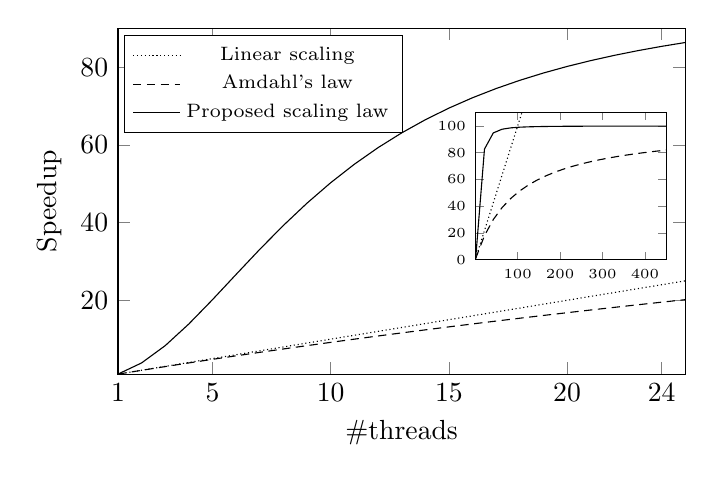
\begin{tikzpicture}[remember picture]
    \begin{axis}[
      width=250pt,
      height=170pt,
      xlabel={\#threads},
      ylabel={Speedup},
      xlabel near ticks,
      ylabel near ticks,
      xmin=1,
      xmax=25,
      ymin=1,
      ymax=90,
      xtick={1,5,10,15,20,24},
      legend style = {
        anchor = north west,
        at = {(rel axis cs:0.01,0.98)},
        font=\scriptsize,
        % draw = none,
      },
      no markers
      ]
      % use TeX as calculator:
      \addplot[domain=1:25,black,densely dotted]{x};
      \addlegendentry{Linear scaling}

      \addplot[domain=1:25,black,densely dashed]{1/(0.01 + (1-0.01)/x)};
      \addlegendentry{Amdahl's law}

      \addplot[domain=1:25,black,solid]{1/(0.01 + (1-0.01)/x^2)};
      \addlegendentry{Proposed scaling law}

      \coordinate (insetPosition) at (rel axis cs:.97,0.25);
      % \addplot[domain=0:15,black,loosely dashed]{1/(0.4 + (1-0.4)/x)};
      % \addlegendentry{Amdahl's law ($\delta=0.4$)}

      % \addplot[domain=0:15,black,loosely dotted]{1/(0.4 + (1-0.4)/x^2)};
      % \addlegendentry{Proposed scaling law for MTF ($\delta=0.4$)}
    \end{axis}
    \begin{axis}[
      at={(insetPosition)},
      anchor={outer south east},
      width=105pt,
      height=85pt,
      tiny,
      % xlabel={\#cores},
      % ylabel={Speedup},
      xmin=1,
      xmax=450,
      ymin=0,
      ymax=110,
      % ytick={1,2,3,4,5},
      no markers]
      \addplot[domain=1:500,black,densely dotted]{x};
      \addplot[domain=1:500,black,densely dashed]{1/(0.01 + (1-0.01)/x)};
      \addplot[domain=1:500,black,solid]{1/(0.01 + (1-0.01)/x^2)};
    \end{axis}
  \end{tikzpicture}
\end{small}

%%% Local Variables:
%%% mode: latex
%%% TeX-master: "../distributed_mrf.tex"
%%% End:

\end{small}
  \caption{Linear scaling, Amdahl's law and the proposed superlinear scaling, for $s=0.01$, where $s$ is the fraction of the execution time inevitably spent in the sequential part of the code. Our proposed scaling law suggests that superlinear scaling is feasible for specific workloads accompanied by a right combination of a load balancer and a self-adjusting data structure.
    The inset shows the asymptotics depicting the saturation of the superlinear scaling of the system.
    }
  \label{fig:amdahl}
\end{figure}

Inherent to Amdahl's law is that no system can scale faster than linear: doubling parallel resources will yield at most two times the performance. Curiously, there have been several reports on faster-than-linear (\emph{superlinear}) scaling experimentally observed in, e.g., database systems \cite{scalability-analyzed, 10.5555/1012889.1012894}, distributed caching \cite{271208, dobb-2}, SDN analytics \cite{sdn-analytitcs}, high-performance computing \cite{556383, 7733347, 6483679}, multi-robot systems \cite{10.1007/978-3-319-77610-1},  parallel search in information retrieval systems \cite{dobb-1, dobb-2}, and large-scale network simulations \cite{10.1145/3627703.3629574} (see full taxonomies in \cite{7733347, 80148}).
% There seem to be two ways to achieve such superlinear speedup \cite{7733347, 80148}: do disproportionately less work in each worker as we scale the system \cite{7733347}, or add more resources per thread \cite{80148}.
% One typical context in which superlinear growth often emerges is distributed caching \cite{271208, 10.5555/1012889.1012894, dobb-2}: the more CPU cores the more (unshared) L1 cache space available to the application, which tends to make memory-bound\slash cache-bound code disproportionately faster \cite{80148} (see an analysis in \S\ref{sec:background}).  
Many authors argue, however, that superlinear scaling is merely a~byproduct of running memory-\slash cache-bound applications on a ``bigger machine'' \cite{80148}, others are concerned that it is hard to generalize beyond a specific set use cases \cite{7733347, 80148}, and some outright dismiss faster-than-linear scaling all together \cite{gunther-hotsos, 10.1016/0167-8191(86)90024-4}, concluding that \emph{``superlinearity, although alluring, is as illusory as perpetual motion''} \cite{10.1145/2773212.2789974}.

In this paper we challenge this view: we show that distributed systems can be methodologically designed for reaching superlinear scaling. Our motivation is that networking applications are often embarrassingly parallel, % with little or no dependency between parallel workers,
which may admit a massive superlinear initial growth phase before scaling eventually and unavoidably blocking on a serial bottleneck.

Our main observation is that, to achieve superlinearity, one has to carefully combine an appropriate load balancing policy with a proper worker implementation. Indeed, load balancing in most distributed systems is deliberately designed to improve the locality of reference in the input of the workers: web apps apply the ``sticky sessions'' rule to route all requests of a particular user to the same web server; %, rendering subsequent requests faster by having all per-user state available locally;
networking code often uses IP 5-tuple hashing on the NIC to ensure that all packets of a flow are processed on the same CPU; % that has local access to per-flow information;
and key-hashing in sharded key-value stores directs all client queries to a key to the same replica. Each of these load balancing policies tend to make the input stream processed by the parallel workers more predictable, compared to the input processed by the system. Such a \emph{locality boosting load balancer}, paired with a \emph{self-adjusting algorithm} so that workers can take advantage of the higher input predictability to adaptively improve their performance, will, as we show both theoretically and empirically, yield faster-than-linear speedup in a broad range of applications (see Fig.~\ref{fig:amdahl}). % One growth factor would come from the self-adjusting algorithm becoming proportionately faster as it processes a smaller and smaller subset of the inputs, and another factor would result from the fact that we throw more CPU resources to the system.

After some background on Amdahl's law (\S\ref{sec:background}), we present our \emph{distributed self-adjusting system architecture} and show that superlinear speedup is a natural product of combining locality-boosting load balancing with self-adjusting algorithms (\S\ref{sec:architecture}). Using common list and tree search algorithms from the literature, we achieve $100$--$3300\times$ speedup in simulations, orders of magnitude surpassing Amdahl's law or even plain, linear scaling. As an unexpected byproduct, we attain linear scaling even when we limit the system to a single CPU core. Then we extend our analysis to real systems (\S\ref{sec:case-study}): we carefully apply our methodology to engineer a Linux-kernel based packet classifier to reach superlinear scaling. On synthetic and real-life firewall traces, our implementation shows up to $800\times$ faster than linear scaling, $5$--$25\times$ improvement beyond the default Linux firewall implementation which scales according to Amdahl's law. Finally, we review related work (\S\ref{sec:related-work}) and draw the conclusions (\S\ref{sec:conclusions}). We note that all code will be available as open source after publication.

%%% Local Variables:
%%% mode: latex
%%% TeX-master: "distributed_mrf"
%%% End:

